\chapter{Metodología de Desarrollo}
\label{chap:metodologia}
%\endinput
 %De acuerdo a \cite{Barrett2009}, el modelo WCM...\\
Para el desarrollo de este trabajo se opt\'o por un modelo de desarrollo de tipo incremental (que resulta iterativo por naturaleza).
En cada iteraci\'on, se optimiz\'o el dise\~no y se fueron agregando nuevas funcionalidades y capacidades al sistema.\\

El problema que se propone resolver, requiere de la implementaci\'on de distintos algoritmos en una estructura en donde los resultados de un m\'odulo se utilizan en el siguiente. Esto implica que para un an\'alisis completo cada una de las instancias debi\'o estar previamente validada.
No obstante, las salidas de los m\'odulos que eran ingesta de otros m\'odulos pod\'ian reemplazarse por datos ya conocidos, y as\'i desarrollar y validar el m\'odulo siguiente, mientras se analizaba en paralelo c\'omo mejorar o corregir los resultados no satisfactorios. De esta manera se fue armando el cuerpo general del software a gran escala, y luego se fue revisando y afinando cada uno de los paquetes.\\

Esta forma de trabajo permiti\'o dividir la complejidad del proyecto, y a su vez, desarrollar un conjunto de bibliotecas f\'acilmente modificables, sin alterar la estructura central.\\

\section{Inicializaci\'on}
En esta primera etapa se evalu\'o  el concepto del ARxCODE en el contexto de la Unidad de Desarrollo de Desechos Espaciales de la CONAE. Fundamentalmente la vinculaci\'on con el departamento de Din\'amica Orbital y los procedimientos actuales que se realizan en relaci\'on a los riesgos de colisi\'on con desechos.

Se hizo un estudio de las estructuras org\'anicas existentes y los sistemas asociados. Los distintos tipos de productos y usuarios, las interfaces que existen y el acceso a los datos reales con los que se  podr\'ia contar.\\

Se analiz\'o c\'omo trabajan otras agencias espaciales el problema de los desechos espaciales y se sacaron conclusiones respecto de qu\'e es lo que podr\'ia ofrecerse y bajo qu\'e premisas.\\

De las consideraciones m\'as importantes que se desprendieron de esta etapa, cabe destacar que se decidi\'o un prototipo para funcionar montado sobre el software principal de Din\'amica Orbital, como un anexo que no interfiere de ninguna manera con los procesos actuales.
Por otro lado, debido a la complejidad del problema y sus consecuencias, ser\'a un software diseñado para ser utilizado por un analista experto, con conocimientos de Din\'amica Orbital.\\

En el mismo sentido, sus productos finales no ser\'an considerados en la toma de decisiones hasta tanto sus resultados no hayan sido validados durante un periodo suficiente, que permita verificar y mejorar su funcionamiento, contrast\'andolo con un acumulado de situaciones reales.\\

Para este planteo de definiciones, se cont\'o con el asesoramiento y el intercambio de informaci\'on con personas del \'area de Din\'amica Orbital y otros departamentos de la CONAE. Se realizaron algunas reuniones e intercambio de correos electr\'onicos, aunque por ser una tem\'atica que se aborda bajo reg\'imenes especiales de acuerdos de confidencialidad, no fue posible contar con la totalidad de la informaci\'on.

\subsection{Plan de Desarrollo}

Dado que el trabajo se realizaba en el contexto de la maestr\'ia en general y que las tareas y los cronogramas se modificaban frecuentemente, ajust\'andose al dictado de cursos y tareas del proyecto integrador que tambi\'en formaba parte del ciclo lectivo; al principio no era posible armar un cronograma fijo de las tareas. Se planific\'o una distribuci\'on horaria (Fig. \ref{fig:disths}) y una planificaci\'on general (Fig. \ref{fig:plan2016}) para los semestres I,III y IV del año 2016.

\begin{figure}[h!]
  \centering
  \fbox{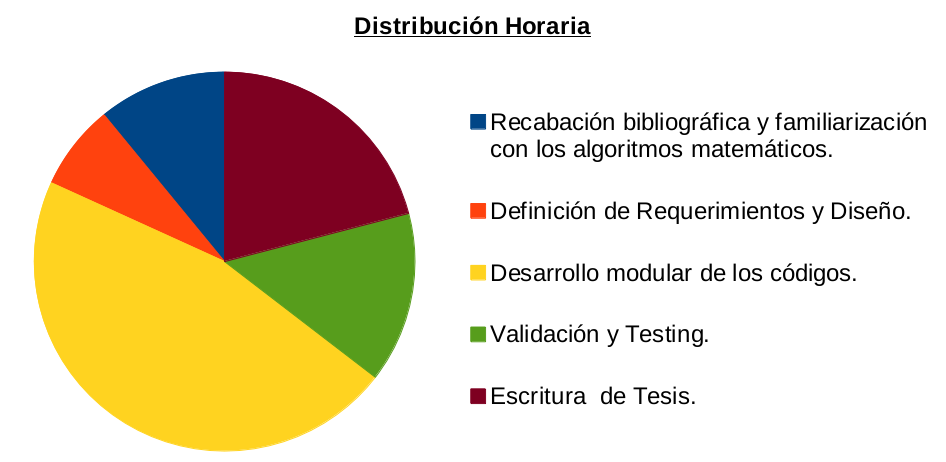
\includegraphics[width=0.7\textwidth]{imagenes/distribucionhs}}
  \caption{Planificaci\'on de la distribuci\'on del total de horas asignadas dentro de la maestr\'ia al desarrollo y la escritura del trabajo de tesis.}
  \label{fig:disths}
\end{figure}

\begin{figure}[h!]
  \centering
  \fbox{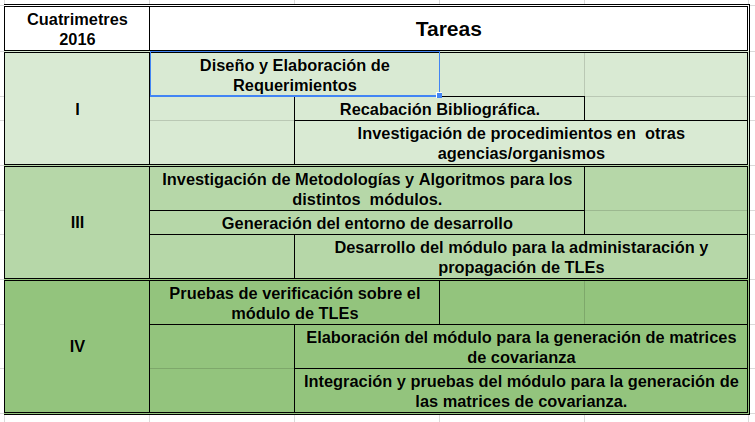
\includegraphics[width=\textwidth]{imagenes/plan2016}}
  \caption{Planificaci\'on de las tareas agrupadas por semestres para el año 2016}
  \label{fig:plan2016}
\end{figure}

Ya a comienzos del año 2017 se contaba con un cronograma fijo que pautaba tres semanas por mes de dedicaci\'on exclusiva a la elaboraci\'on de la tesis. Eso permiti\'o realizar una planificaci\'on semanal (Fig. \ref{fig:plan2017}) de las tareas. 

\begin{figure}[h!]
  \centering
  \fbox{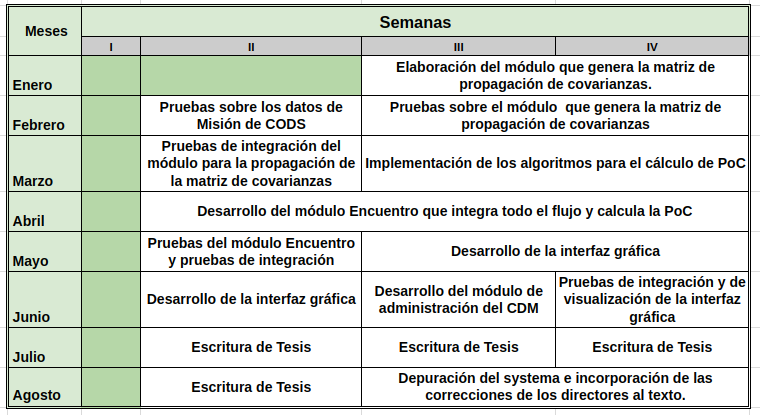
\includegraphics[width=\textwidth]{imagenes/plan2017}}
  \caption{Planificaci\'on de las tareas agrupadas por semanas para el año 2017}
  \label{fig:plan2017}
\end{figure}

\section{Iteraci\'on}
Ya conocido el planteo del problema, las distintas maneras de abordarlo y las restricciones, se elabor\'o un diseño preliminar del producto con sus requerimientos (Sec. \ref{sec:requerimientos}) y sus funcionalidades, que dadas las caracter\'isticas del problema result\'o bastante determinista.\\

Para el desarrollo se definieron distintos paquetes o componentes (Sec. \ref{subsec:componentes}):\\

\begin{itemize}
\itemsep0em
 \item Paquetes de Procesamiento: {\it{AjustarTle}}, {\it{Comparar}}, {\it{Encuentro}}, {\it{Estad\'istica}}.
 \item Paquetes de Administraci\'on de Datos: {\it{TleAdmin}}, {\it{CodsAdmin}}, {\it{CDM}}.
 \item Paquetes Generales de utilizaci\'on m\'ultiple: {\it{SistReferencia}}, {\it{Validaci\'on}}.
 \item Paquetes de visualizaci\'on e interfaz gr\'afica: {\it{Aplicaci\'on}}, {\it{visual}}.
\end{itemize}

Esta metodolog\'ia permiti\'o importar funciones que resuelven cuestiones espec\'ificas desde cualquier  m\'odulo y a su vez modificar las funciones cuando fuera necesario.\\

Durante el diseño y el desarrollo de la interfaz, se fueron modificando mucho las opciones, en tanto se utiliz\'o la interfaz para seguimiento de pasos intermedios que a medida que iban siendo verificados se iban retirando de las opciones del usuario.\\

\section{Seguimiento y Control}

\subsection{Verificaci\'on y Validaci\'on}

\subsubsection*{Verificaci\'on}
Se realizaron distintas pruebas de unidad y de integraci\'on.  
Los distintos casos de prueba se diseñaban a partir de datos de prueba de la bibliograf\'ia recabada para cada una de las metodolog\'ias o sobre situaciones reales. Los resultados de la ejecución de las pruebas se comparaba luego con los valores de  los casos publicados \ref{fig:metodoprueba}. 

\begin{figure}[h!]
  \centering
  \fbox{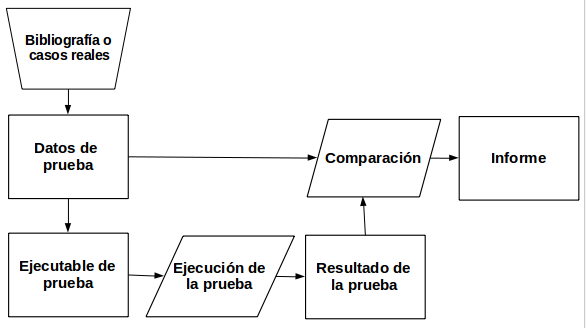
\includegraphics[width=0.7\textwidth]{imagenes/metodoprueba}}
  \caption{Esquema de la metodología para realizar las pruebas de unidad sobre los módulos.}
  \label{fig:metodoprueba}
\end{figure}

A medida que se desarrollaba un nuevo m\'odulo, se realizaban los casos de prueba para ese m\'odulo y una prueba de integraci\'on, que incorporaba todos los m\'odulos hasta el momento verificados.

\paragraph*{TleAdmin y CDM}
Dado que tanto los TLE como los CDM son los elementos fundamentales que dan inicio al an\'alisis de la probabilidad de colisi\'on, es fundamental tener un control sobre la correcta adquisici\'on de estos inputs. Sobre ellos se diseñaron pruebas funcionales. Se prueba siempre que los TLE de ambos objetos hayan sido adquiridos; si esto no fuera as\'i ya sea por complicaciones en la conexi\'on a internet, o porque los TLE para las fechas solicitadas no est\'an disponibles, el software interrumpe el proceso e indica a cu\'al de las situaciones se debe el problema. Mientras que para el caso de los CDM, el programa se interrumpe si el archivo ingresado no respeta el formato .xml capaz de procesar y anuncia un mensaje de alerta cuando el CDM a sido procesado pero no todos los campos de inter\'es se encuentran en \'el. 

\paragraph*{Comparar y SistReferencia}
Las pruebas realizadas para garantizar los correctos procedimientos respecto de la propagaci\'on y las transformaciones de los sistemas de referencia fueron fundamentales, pero s\'olo se realizaron en las primeras etapas del desarrollo, ya que no dependen de cada ejecuci\'on en particular, sino de la correcta implementaci\'on de los algoritmos.  

\paragraph*{Estad\'istica}
Para verificar la correcta implementaci\'on del m\'etodo de Osweiler para la generaci\'on de las matrices de covarianza, se gener\'o un caso de prueba que permite comparar los resultados con los que se publican en el trabajo del autor. Dada la dependencia de este m\'odulo con el m\'odulo de administraci\'on de los TLE, es importante que esta prueba es naturalmente de integraci\'on y es muy importante que se realice frecuentemente. ! LA DIAGONAL DE LA MATRIZ DEBE SER POSITIVA. 

\paragraph*{Comparar y CodsAdmin}
El procedimiento que se realiza para la generaci\'on de la matriz de propagaci\'on de errores involucra la utilizaci\'on de los datos de misi\'on (o Datos de CODS). Esta tarea fue realmente compleja y se realizaron varias ejecuciones de la prueba sobre la manipulaci\'on de estos datos, ya que los mismos muchas veces no respetaban un formato estandarizado por ejemplo sobre las fechas o conten\'ian intervalos sin datos significativos, etc. Estas verificaciones se realizaron una sola vez hasta lograr que los datos resultaran ordenados dentro del per\'iodo de an\'alisis que se utiliz\'o para generar la matriz de propagaci\'on de errores. Por cuestiones de tiempo no se implement\'o una verificaci\'on automatizada sobre estos inputs, lo que debe ser tenido en cuenta si se desean generar matrices de propagaci\'on de errores actualizadas o en forma din\'amica.  

\paragraph*{Encuentro}
Las pruebas realizada en el m\'odulo para la estimaci\'on de las probabilidades de colisi\'on tienen tambi\'en una fuerte dependencia del m\'odulo que gestiona los TLE, mientras que pueden configurarse o no para que la matriz de covarianza que utilizan sea generada por el m\'odulo de Osweiler o no. Salvo para el caso del m\'etodo de Lei-Chen, ya que en su trabajo existe un ejemplo que indica todos los par\'ametros que se utilizan en la ecuaci\'on final, y entonces se puede hacer una prueba s\'olo para esa unidad.

\paragraph{Aplicaci\'on}
En lo que respecta a la aplicaci\'on que nuclea y despliega la interfaz gr\'afica, se realizaron inspecciones para depurar la correcta inicializaci\'on de variables y el flujo de las distintas vistas. 


\begin{figure}[!h]
\begin{minipage}[t]{0.48\textwidth}
 \centering
 \fbox{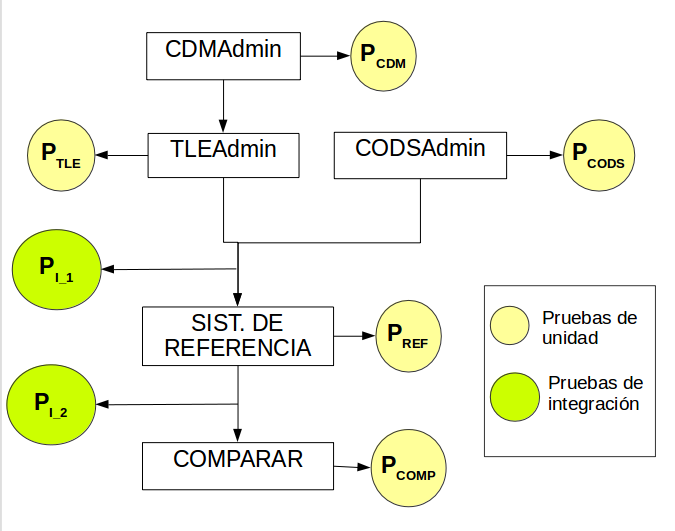
\includegraphics[width=0.9\textwidth]{imagenes/pruebasCods}}
 \caption[Casos de Prueba I]{Casos de prueba para los módulos que interactúan con los datos de Misión.}
 \label{fig:pruebaCods}
\end{minipage}
\begin{minipage}[t]{0.48\textwidth}
 \centering
 \fbox{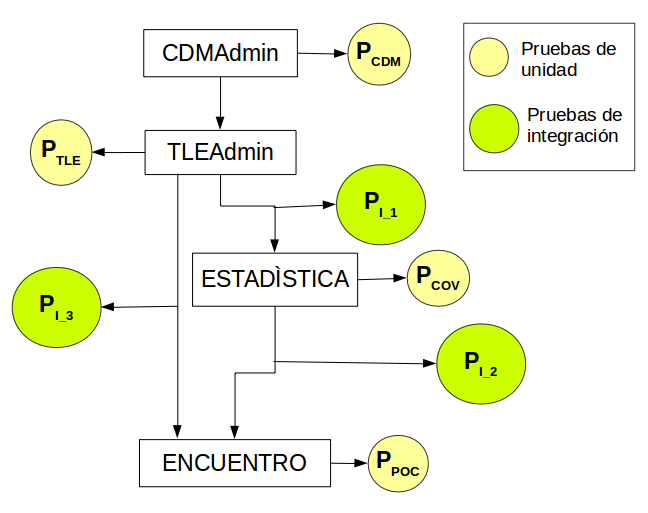
\includegraphics[width=0.9\textwidth]{imagenes/pruebasEncuentro}}
 \caption[Casos de Prueba II]{Casos de prueba del bloque completo, desde los inputs hasta el cálculo de la PoC.}
 \label{fig:pruebaEncuentro}
\end{minipage}
\end{figure}

\subsubsection*{Validaci\'on}

Al tratarse de un sistema que implementa distintas metodolog\'ias para el c\'alculo de par\'ametros, el control m\'as exhaustivo se bas\'o en analizar que los resultados de los algoritmos implementados fueran coherentes y coincidieran con los que exist\'ian en publicaciones bibliogr\'aficas o situaciones reales que se pod\'ian reproducir. \\

En conclusi\'on se han realizado distintas pruebas e inspecciones, pero no pruebas exhaustivas.
Un desarrollo detallado de los resultados de las pruebas y validaciones se describe en la Sec. \ref{chap:resultados}\\

\subsection{Gesti\'on de la Configuraci\'on}

Al ser ARxCODE un prototipo sencillo desarrollado por una sola persona, no fue necesario implementar una compleja gesti\'on de configuraci\'on. Se utiliz\'o el repositorio Git (Ver Sec. \ref{sec:entorno}) para el control de versiones, al que d\'ia a d\'ia se incorporaba el proyecto. Se paut\'o realizar un release una vez por mes, ya que era la frecuencia con la que se planific\'o que existieran nuevos m\'odulos y pruebas de unidad y/o de integraci\'on. 


\subsection{Aseguramiento de la Calidad}

\begin{itemize}
 \item Que los TLE no se aparten demasiado de la fecha predicha
 \item Que los CDMs provengan en el formato estandarizado CCSDS
 \item Que el modelo de propagaci\'on sea bueno
 \item Que las matrices de covarianza contengan errores acotados. 
 \item Que los m\'etodos implementados en el c\'alculo de la PoC sean los aceptados
 \item Que los c\'alculos de las distintas ecuaciones se realicen correctamente en todos los casos
\end{itemize}



\section{Entorno de Desarrollo}\label{sec:entorno}

Para el desarrollo se utiliz\'o:\\
\begin{itemize}
 \item Plataforma de Desarrollo (\ac{IDE}): Eclipse Ver. 3.8.1.
 \item Lenguaje de Programaci\'on: Python 2.7
 \item Biblioteca de Interfaz gr\'afica: QT por medio del enlace PyQT.
 \item Gestor de Configuraci\'on: Git.
\end{itemize}

\subsection*{Eclipse}
Eclipse (Ver. 3.8.1) es una plataforma de desarrollo multiplataforma ampliamente utilizada y ya muy madura, cuya estructura de perspectivas, editores y vistas, facilita el desarrollo en distintos lenguajes de programaci\'on. En este trabajo se incorpor\'o el IDE para python, {\it{Pydev}}.\\

Eclipse ofrece excelentes capacidades para la gesti\'on de proyectos, permitiendo incorporar en un mismo proyecto distintos archivos y documentaci\'on, que, en esta tesis, agrup\'o no s\'olo los datos de entrada y salida, como los TLE, los CDM o los productos orbitales; sino que tambi\'en incluy\'o todos los ploteos y gr\'aficos que resultaban de los procesamientos y la propia documentaci\'on referida a la escritura de este documento. Esto fue muy productivo en lo que respecta al control de versiones, ya que se aprovech\'o el hecho de que Eclipse ya tiene incorporado el gestor Git.
Cabe destacar también, que cuenta con una excelente herramientas de depuraci\'on.\\

\subsection*{Python}
El lenguaje de programaci\'on Python se destaca en sus capacidades tanto de c\'alculo como de manejo de texto. Esto agiliza mucho los procesos que involucran el manejo de tablas de datos plasmadas en texto plano, como son por ejemplo los datos TLE y las efem\'erides orbitales que se generan como productos del departamento de Din\'amica Orbital. As\'i mismo facilita el manejo de las nomenclaturas de los distintos archivos de datos o im\'agenes generadas.\\

Existen numerosas, potentes y optimizadas bibliotecas para la realizaci\'on de c\'alculos, y el tratamiento vectorial. En nuestro caso se aprovech\'o particularmente la biblioteca {\it{numpy}}, y muy poco de {\it{scipy}} espec\'ificamente, para interpolar datos.
Finalmente su utilizaci\'on masiva permite tener acceso r\'apido a sus potencialidades.\\

\subsection*{QT}
Para el desarrollo de la interfaz gr\'afica se utiliz\'o QT, a trav\'es del enlace PyQT.\\
QT es un framework ampliamente utilizado para el desarrollo de aplicaciones multiplataforma. Cuenta con mucha contribuci\'on de la comunidad y est\'a soportado por Nokia.\\

Su mecanismo de conexión de señales y eventos es simple, esto permite definir los eventos sencillos en la estructura del GUI, y luego invocar el c\'odigo python con las acciones m\'as avanzadas. Subyace su implementaci\'on en C++ que muchas veces dificulta la comprensi\'on para los que estamos familiarizados con la l\'ogica del python, y lo mismo ocurre con la documentaci\'on y prevalecen los ejemplos para C++.\\

\subsection*{Git}
Si bien, esta herramienta no fue aprovechada en todo su potencial en este trabajo, por tratarse de un proyecto sencillo y desarrollada por dos personas, fue fundamental para agilizar la posibilidad de trabajar desde cualquier computadora, siempre en la \'ultima versi\'on del proyecto.
As\'i mismo, el trabajo con control de versiones, permiti\'o realizar distintas pruebas e implementaciones que luego se descartaron o se quitaron del producto final, pero que pueden ser reutilizados en futuros proyectos. En particular, en la utilizaci\'on de la interfaz intermedia que fue generada para una \'agil evaluaci\'on de los resultados parciales.\\









